\documentclass[a4paper,11pt]{article}

\usepackage[utf8]{inputenc}

\usepackage{graphicx}
\usepackage{caption}
\usepackage{subcaption}

\usepackage{hyperref}

\usepackage{pgfplots}
\pgfplotsset{compat=1.18} 

\usepackage{minted}

\begin{document}

\title{
    \textbf{Assignment 12 Report - Graphs in Java}
}
\author{Dean Tsankov}
\date{\today}

\maketitle

\section*{Introduction}

In this report I will present one of the more general linked data structures. A graph is a set of vertices connected through edges with each other. The edges can be used to represent paths that connect points that are not directly connected and thus make the graph traversible in some sense. A few of the data structures we have already discussed fall into the category of graphs, such as trees and the linked list type structures. Here we will explore the most general sort of graph i.e. we let go of any restrictions on the structure unlike the mentioned previously explored themes.
\\

In order to visualize the operations over the graph we will be using a set of cities in Sweden connected to each other via train lines. Each connection between two cities is given to us in a CSV formatted file along with the respective time it takes to travel the distance.

\section*{Populating the graph with data}

The first task we have is to structure the provided set of data into a useful to us graph. First some underlying classes are defined. Those are the City and Connection classes. 
\\

A city has a name and a list of connections representing all other cities it has direct train lines to. 
\begin{minted}[
frame=single,
framesep=2mm,
baselinestretch=1.2,
fontsize=\footnotesize,
]{java}
    (...)
    public class City {
        String name;
        ArrayList<Connection> conections;

        public City(String name) {
            this.name = name;
            this.conections = new ArrayList<Connection>();
        }
        
        public void connect(City nxt, int dst) {
            this.conections.add(new Connection(nxt, dst));
        }
    }
    (...)
\end{minted}

A connection stores a city destination as well as the time to reach it. 
\begin{minted}[
frame=single,
framesep=2mm,
baselinestretch=1.2,
fontsize=\footnotesize,
]{java}
    (...)
    public class Connection {
        City destination;
        int timeToReach;

        public Connection(City destination, int timeToReach) {
            this.destination = destination;
            this.timeToReach = timeToReach;
        }
    }
    (...)
\end{minted}

We then go line by line in the CSV file and create the two city vertices or nodes if they have not yet been created, represented by the entry and then "connect" them. Here all links are bidirectional which means that if city A is connected to B then B is also connected to A. The class responsible for initializing the graph then only needs to have properties for the array of cities in the set. But then since we would like this class to provide us with a quick lookup method we would turn this array into a hash table implemented with buckets. Its constructor then has the form:

\begin{minted}[
frame=single,
framesep=2mm,
baselinestretch=1.2,
fontsize=\footnotesize,
]{java}
    (...)
    public Map(String file) {
        this.cities = new City[mod];
        this.buckets = (ArrayList<City>[]) new ArrayList[mod];

        try (BufferedReader br = new BufferedReader(new FileReader(file))) {
            String line;
            while ((line = br.readLine()) != null) {
                String[] row = line.split(",");
                City one = lookup(row[0]);
                City two = lookup(row[1]);
                int dist = Integer.valueOf(row[2]);

                one.connect(two, dist);
                two.connect(one, dist);

            }
        } catch (Exception e) {
            System.out.println(e.getMessage());
        }
    }
    (...)
\end{minted}
We want to lookup each city and that makes sure that if the city is already in the graph we only add a connection to it and do not add duplicates with the same name. The lookup method is a bit complex, but does the bulk of the work to setup the proper structure of the graph.

\begin{minted}[
frame=single,
framesep=2mm,
baselinestretch=1.2,
fontsize=\footnotesize,
]{java}
    (...)
    public City lookup(String name) {
        int hashedIndex = hash(name, this.mod);
        if (cities[hashedIndex] != null) {
            if (cities[hashedIndex].name.equals(name)) {
                return cities[hashedIndex];
            }else if (buckets[hashedIndex] == null){
                buckets[hashedIndex] = new ArrayList<City>();
                City res = new City(name);
                buckets[hashedIndex].add(res);
                return res;
            }else if(!buckets[hashedIndex]
                    .stream()
                    .anyMatch(c -> c.name == name)) {
                City res = new City(name);
                buckets[hashedIndex].add(res);
                return res;
            } else {
                return buckets[hashedIndex]
                        .stream()
                        .filter(c -> c.name == name)
                        .findFirst()
                        .orElse(null);
            }
        } else {
            cities[hashedIndex] = new City(name);
        }

        return cities[hashedIndex];
    }
    (...)
\end{minted}
It is very similar in a way to the lookup method implemented in the Hash tables assignment, but now also adds the city node if it is nowhere to be find in the array or its bucket list.

\section*{A Naive way to find the shortest path between cities}
One very naive solution, when we think about it, to find the shortest path between two cities is to perform a depth first search over the graph beginning from one of the cities and checking in depth the shortest way to reach the other. This has some pit holes we should consider first, though. Knowing that the links are bidirectional it is not hard to notice that it would be very easy to enter an infinite spiral where we go through the same cities without making any progress in our search algorithm. To negate this we should implement a maximum distance traveled constraint, which subtracts the connection's distance each time we traverse it and when the constraint reaches zero we finish the execution. 
\\

Filling in the following loop segment in the provided {\tt shortest()} method will make it usable:

\begin{minted}[
frame=single,
framesep=2mm,
baselinestretch=1.2,
fontsize=\footnotesize,
]{java}
    (...)
    for (Map.Connection c : from.conections) {
        if (c != null) {
            Integer currDist = shortest(c.destination, 
                    to, max - c.timeToReach);
            if (currDist != null) {
                Integer distSum = c.timeToReach + currDist;
                if (shrt == null || distSum < shrt) {
                    shrt = distSum;
                }
            }
        }
    }
    (...)
\end{minted}

\subsection*{Benchmarking}

We are asked to try and run the search for shortest path algorithm on a couple of pairs of cities. But as it should become clear this solution, while functional in theory, becomes quite cumbersome in practice, judging from the couple of x values in the table, of timed out executions. This is due to an underlying exponential complexity of the traversal.

\begin{table}[H]
\begin{center}
\begin{tabular}{l|c|c}
\textbf{Route} & \textbf{Travel time (min)} & \textbf{Execution time (ms)}\\
\hline
  Malmö to Göteborg      &  153 &     3 \\
  Göteborg to Stockholm       &  211 &    4 \\
  Malmö to Stockholm  &  273 &   4 \\
  Stockholm to Sundsvall  &  327 &   439 \\
  Stockholm to Umeå  &  x &   411 \\
  Göteborg to Sundsvall  &  x &   1501 \\
  Sundsvall to Umeå  &  190 &   1 \\
  Umeå to Göteborg  &  705 &   1505 \\
  Göteborg to Umeå  &  x &   1544 \\
\end{tabular}
\caption{Graph DFS benchmark}
\label{tab:table1}
\end{center}
\end{table}

Spending a bit of time thinking about how our algorithm works currently, makes us realize that there are a lot of multiples of the same operations done over and over again without getting us closer to the result. This happens of course due to the before mentioned loops. A max restraint limits their effect, but does not in any way prevent them from happening in the first place.

\section*{Keeping track of the path taken}

We implement a separate array of cities which will keep track of the ones we have already been to during our search and as such when we decide to go along a link we will have to check if we already went to the linked city or not yet. Since the {\tt shortest()} method is implemented recursively this path array of cities will perform much like a stack and we will keep track of a stack pointer index in order to push and pop cities onto it as we visit them. 

The function now looks like this:

\begin{minted}[
frame=single,
framesep=2mm,
baselinestretch=1.2,
fontsize=\footnotesize,
]{java}
    (...)
    private Integer shortest(Map.City from, Map.City to) {
        if (from.equals(to)) {
            return 0;
        }
        
        Integer shrt = null;

        for (int i = 0; i < sp; i++) {
            if (path[i] == from)
            return null;
        }
        path[sp++] = from;
        for (Map.Connection c : from.conections) {
            if (c != null) {
                Integer currDist = shortest(c.destination, to);
                if (currDist != null) {
                    Integer distSum = c.timeToReach + currDist;
                    if (shrt == null || distSum < shrt) {
                        shrt = distSum;
                    }
                }
            }
        }
        path[sp--] = null;
        return shrt;
    }
    (...)
\end{minted}

Performing the same benchmark tests now gives nicer results and all travel times are able to be computed.

\begin{table}[H]
\begin{center}
\begin{tabular}{l|c|c}
\textbf{Route} & \textbf{Travel time (min)} & \textbf{Execution time (ms)}\\
\hline
    Malmö to Göteborg  &  153 &   16 \\
    Göteborg to Stockholm  &  211 &   1 \\
    Malmö to Stockholm  &  273 &   2 \\
    Stockholm to Sundsvall  &  327 &   3 \\
    Stockholm to Umeå  &  517 &   4 \\
    Göteborg to Sundsvall  &  515 &   4 \\
    Sundsvall to Umeå  &  190 &   8 \\
    Umeå to Göteborg  &  705 &   4 \\
    Göteborg to Umeå  &  705 &   5 \\
    Malmö to Kiruna  &  1162 &   19 \\
\end{tabular}
\caption{Graph DFS benchmark}
\label{tab:table1}
\end{center}
\end{table}

\subsection*{Improving further}

Even still there is another optimization we can implement in hopes of lowering execution even further. We could change the max constraint dynamically. It begins as null, but as soon as we find a path to the destination we know that the one we are searching for will always be no larger than the one we just found, so we set the constraint to that value. This means that with each step along the graph we refine this value until we find our result.
\\

The changes to the new shortest function are as follow:

\begin{minted}[
frame=single,
framesep=2mm,
baselinestretch=1.2,
fontsize=\footnotesize,
]{java}
    (...)
    if (max!=null && max < 0){
        return null;
    }
    (...)
    for (Map.Connection c : from.conections) {
        if (c != null) {
            if (max != null) {
                max -= c.timeToReach;
            }
            Integer currDist = shortest(c.destination, to, max);
            if (currDist != null) {
                Integer distSum = c.timeToReach + currDist;
                if (shrt == null) {
                    shrt = distSum;
                }
                if (distSum < shrt) {
                    shrt = distSum;
                    max = shrt;
                }
            }
        }
    }
    (...)
\end{minted}

\subsection*{Comparison}

Pinning the three versions over the set of city to city benchmarks yields the chart:

\pgfplotstableread[row sep=\\,col sep=&]{
    interval & carT & carD & carR \\
    T1  &  3 &   16 &  11 \\
    T2  &  4 & 1 &   3 \\
    T3  &  4 &   2 &   2\\
    T4  &  439 &   3 &   3 \\
    T5  &  411 &   4 &   4 \\
    T6  &  1501 &   4 &   2 \\
    T7  &  1 &   8 &   9 \\
    T8  &  1505  &   4 &   2 \\
    T9  &  1544 &   5 &   2 \\
    T10  &  154 &   19 &   11 \\
    }\mydata

    \begin{tikzpicture}
    \begin{axis}[
            ybar,
            bar width=.25cm,
            width=\textwidth,
            height=.5\textwidth,
            legend style={at={(0.5,1)},
                anchor=north,legend columns=-1},
            symbolic x coords={T1, T2, T3, T4, T5, T6, T7, T8, T9, T10 },
            xtick=data,
            nodes near coords,
            nodes near coords align={vertical},
            ymin=0,ymax=35,
            ylabel={Execution in ms},
        ]
        \addplot table[x=interval,y=carT]{\mydata};
        \addplot table[x=interval,y=carD]{\mydata};
        \addplot table[x=interval,y=carR]{\mydata};
        \legend{Naive, Path track, Path track + dynamic max}
    \end{axis}
\end{tikzpicture}

We can notice that our considerations do pay off, but the fact of the matter is that this depth first search for the shortest distance algorithm still has exponential time complexity and would definitely not fare well for larger data sets.  

\begin{figure}[H]
    \centering
    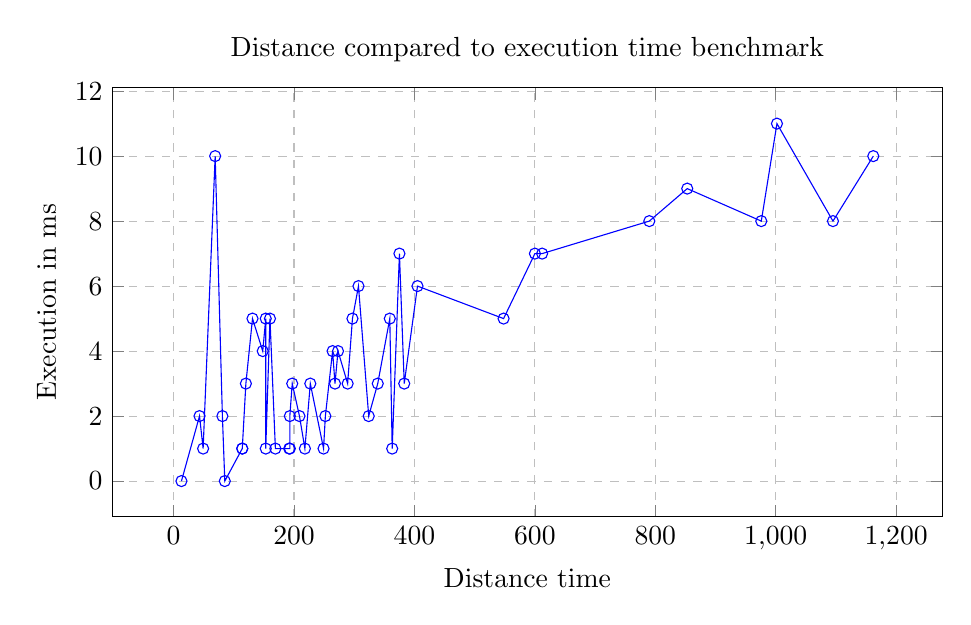
\begin{tikzpicture}
        \begin{axis}[
            title={Distance compared to execution time benchmark},
            width=\linewidth,
            height=200,
            xlabel={Distance time},
            ylabel={Execution in ms},
            ymajorgrids=true,
            xmajorgrids=true,
            grid style=dashed,
        ]
        

        \addplot[
            color=blue,
            mark=o,
            ]
            coordinates {
            (13, 0)(43, 2)(49, 1)(69, 10)(81, 2)(85, 0)(114, 1)(114, 1)(120, 3)(131, 5)(148, 4)(153, 5)(153, 1)(160, 5)(169, 1)(192, 1)(193, 1)(193, 2)(197, 3)(209, 2)(218, 1)(227, 3)(249, 1)(252, 2)(264, 4)(268, 3)(273, 4)(289, 3)(297, 5)(307, 6)(324, 2)(339, 3)(359, 5)(363, 1)(375, 7)(383, 3)(405, 6)(548, 5)(600, 7)(612, 7)(790, 8)(853, 9)(976, 8)(1002, 11)(1095, 8)(1162, 10)
            };
            
            
        \end{axis}
        \end{tikzpicture}
    \caption{Distance compared to execution time benchmark}
    \label{fig:plot1}
\end{figure}
 With this last graph I tried to show the exponential growth of the execution time with respect to the distance traversed using our most optimized solution so far. To what extent it serves its purpose is questionable. Nevertheless, this was done by computing the shortest distance from Malmö to every other city in the data set and then sorting the results in ascending order based on the distance. The code for this benchmark can be found in the respective \href{https://github.com/kexana/Algorithms-and-Data-Structures-ID1021}{github} repository for the assignment.

 \section*{Closing}
All in all we now have a solution that works for the small data, but will be
very inefficient for larger maps. A large problem with the current algorithm is that it does not in any way keep track of previously performed computations. Finding a way to record our previous work will be key to reaching optimal performance.
 

\end{document}

